\documentclass[11pt, a4paper]{article}

% --- Encoding, Language, Style ---
\usepackage[utf8]{inputenc}
\usepackage[T1]{fontenc}
\usepackage[english]{babel}
\usepackage[scaled=0.92]{helvet}

% --- Layout ---
\usepackage[top=2.5cm, bottom=2.5cm, left=1cm, right=1cm]{geometry}
\usepackage{titlesec}
\usepackage{fancyhdr}
\usepackage{tabularx}
\usepackage{booktabs}
\usepackage{graphicx}


% --- Metadata ---
\newcommand{\projecttitle}{DHBWay}
\newcommand{\docversion}{Final Version}
\newcommand{\docauthor}{Nicken Labs \\ \vspace{0.5em} \\ Nikolai Schlosser, Julien Armbruster\\ Ben Hibinger, Niklas Reutter}
\newcommand{\docorg}{DHBW Ravensburg -- Campus Friedrichshafen}
\newcommand{\docdate}{\today}

% --- Head- and Footnotes ---
\pagestyle{fancy}
\fancyhf{}
\renewcommand{\headrulewidth}{0pt}
\fancyhead[L]{\textit{\textbf{Inception for \projecttitle}}}
\fancyhead[R]{\textit{\textbf{Page \thepage}}}

% --- Headline formatting---
\titleformat{\section}
  {\normalfont\Large\bfseries}{\thesection.}{0.8em}{}
\titleformat{\subsection}
  {\normalfont\large\bfseries}{\thesubsection}{0.8em}{}
\titleformat{\subsubsection}
  {\normalfont\normalsize\bfseries}{\thesubsubsection}{0.8em}{}

\begin{document}

% ==============================================================================
% Ttile page
% ==============================================================================
\begin{titlepage}
    \sffamily
    \noindent\rule{\textwidth}{3pt}
    \vspace{1.2cm}
    
    \begin{flushright}
        {\fontsize{28}{34}\selectfont\bfseries Inception\par}
        \vspace{1.2cm}
        {\Large\bfseries for\par}
        \vspace{1.2cm}
        {\fontsize{24}{30}\selectfont\bfseries \projecttitle\par}
        \vspace{1.8cm}
        {\large\bfseries \docversion\par}
        \vspace{1.2cm}
        {\large\bfseries Prepared by \docauthor\par}
        \vspace{1.2cm}
        {\large\bfseries \docorg\par}
        \vspace{1.2cm}
        {\large\bfseries \docdate\par}
    \end{flushright}
\end{titlepage}

% --- 1. PROBLEM STATEMENT ---
\section{Problem Statement}
The DHBW Ravensburg Campus Friedrichshafen consists of three buildings (H, N and E).
For people who are new to the campus, such as first-semester students and external
lecturers, it is often hard to find the right room, which leads to delays and
confusion before lectures.\\
In addition, students who want to study between or after lectures do not know which
rooms are currently free, because the timetable only shows where lectures take place.\\
Organising a study group is difficult aswell, since classmates, a common time slot and
a free room all have to be found separately, usually through private chats.\\
Together, these problems cost students and lecturers time every day and make campus
life less efficient than it needs to be.



% --- 2. MOTIVATION ---
\section{Motivation}
The following benefits motivate the development of DHBWay.

\begin{itemize}
    \item \textbf{Less time lost:} New students, external lecturers and staff find their room right away instead of searching or asking around.
    \item \textbf{Better use of rooms:} Free rooms become visible and can be used for study groups or individual work.
    \item \textbf{One place for the day:} Timetable, room and route are shown together instead of looking them up separately.
    \item \textbf{Learning together:} Study groups can be opened and joined easily, which makes it simpler to learn with others.
\end{itemize}

% --- 3. DESCRIPTION OF THE PROPOSED SOLUTION ---
\section{Description of the Proposed Solution}
We propose \textbf{DHBWay}, a web app that helps students and lecturers find their way around the campus and organise their day. It combines an interactive map of the campus with the personal timetable. Users see where their next lecture takes place, get directions to the room and can check which rooms are currently free. Free rooms can be reserved, and users can create study groups that other students can join.

\subsection*{High-Level Concept}
DHBWay is a client-server system. The client runs in the web browser, so it works on laptops and smartphones without building a separate app for every platform. For mobile use, the web app can additionally be wrapped as an app for iOS and Android. The server stores the campus map and the timetable data and provides them to the clients. The timetables are taken from the existing DHBW timetables, so nobody has to maintain them twice.

\subsection*{Core Capabilities (High-Level)}
\begin{itemize}
    \item \textbf{Interactive campus map:} Shows the buildings, floors and rooms of the campus, optionaly as a 3D model.
    \item \textbf{Room navigation:} Guides the user to a selected room.
    \item \textbf{Personal timetable:} Users select their course and see their own timetable. Each lecture is linked to its room, so the navigation can be started directly from the timetable.
    \item \textbf{Room availability:} Combines all timetables to show which rooms are free at a given time. A free room can be reserved.
    \item \textbf{Study groups:} Users can create a study group. Other students can browse the groups and join them. If a member reserves a room, the group gets a notification.
    \item \textbf{Intuitive UI:} Using the App is intuitive and fast.
\end{itemize}

% --- 4. EXPECTED STAKEHOLDERS ---
\section{Expected Stakeholders}

\begin{itemize}
    \item \textbf{Students:} They want to find rooms quickly, see which rooms are free
    and plan study groups easily. They expect the app to be simple and fast to use.

    \item \textbf{Lecturers (internal and external):} They want to find their lecture
    rooms without searching. External lecturers who are rarely on campus profit the most.

    \item \textbf{Study Program Management and Secretariat:} They create the timetables
    in Rapla. The app has to use this data correctly and must not change it.

    \item \textbf{Development Team:} We build and maintain the app. Our constraints are
    the limited time of the project and our technical knowledge.
\end{itemize}

% --- 5. INTENDED USERS ---
\section{Intended Users}
DHBWay is intended for everyone who needs to find their way around the campus or wants to use its rooms for studying. 
\vspace{1em}

\noindent
\begin{tabularx}{\textwidth}{l X X}
    \toprule
    \textbf{User Role (Actor)} & \textbf{Profile / Context} & \textbf{Primary Goals in the System} \\
    \midrule
    \textbf{Student} & Studies at the campus. First-semester students do not know the buildings H, N and E yet& Navigate to lecture rooms, find free rooms for self-study, view their own timetable, create or join study groups \\
    \addlinespace
    \textbf{External lecturer} & Teaches only a few lectures and rarely visits the campus & Find the assigned lecture room without having to ask around \\
    \bottomrule
\end{tabularx}


% --- 6. INITIAL USE-CASE DIAGRAMS ---
\section{Initial Use-Case Diagram}
\begin{center}
  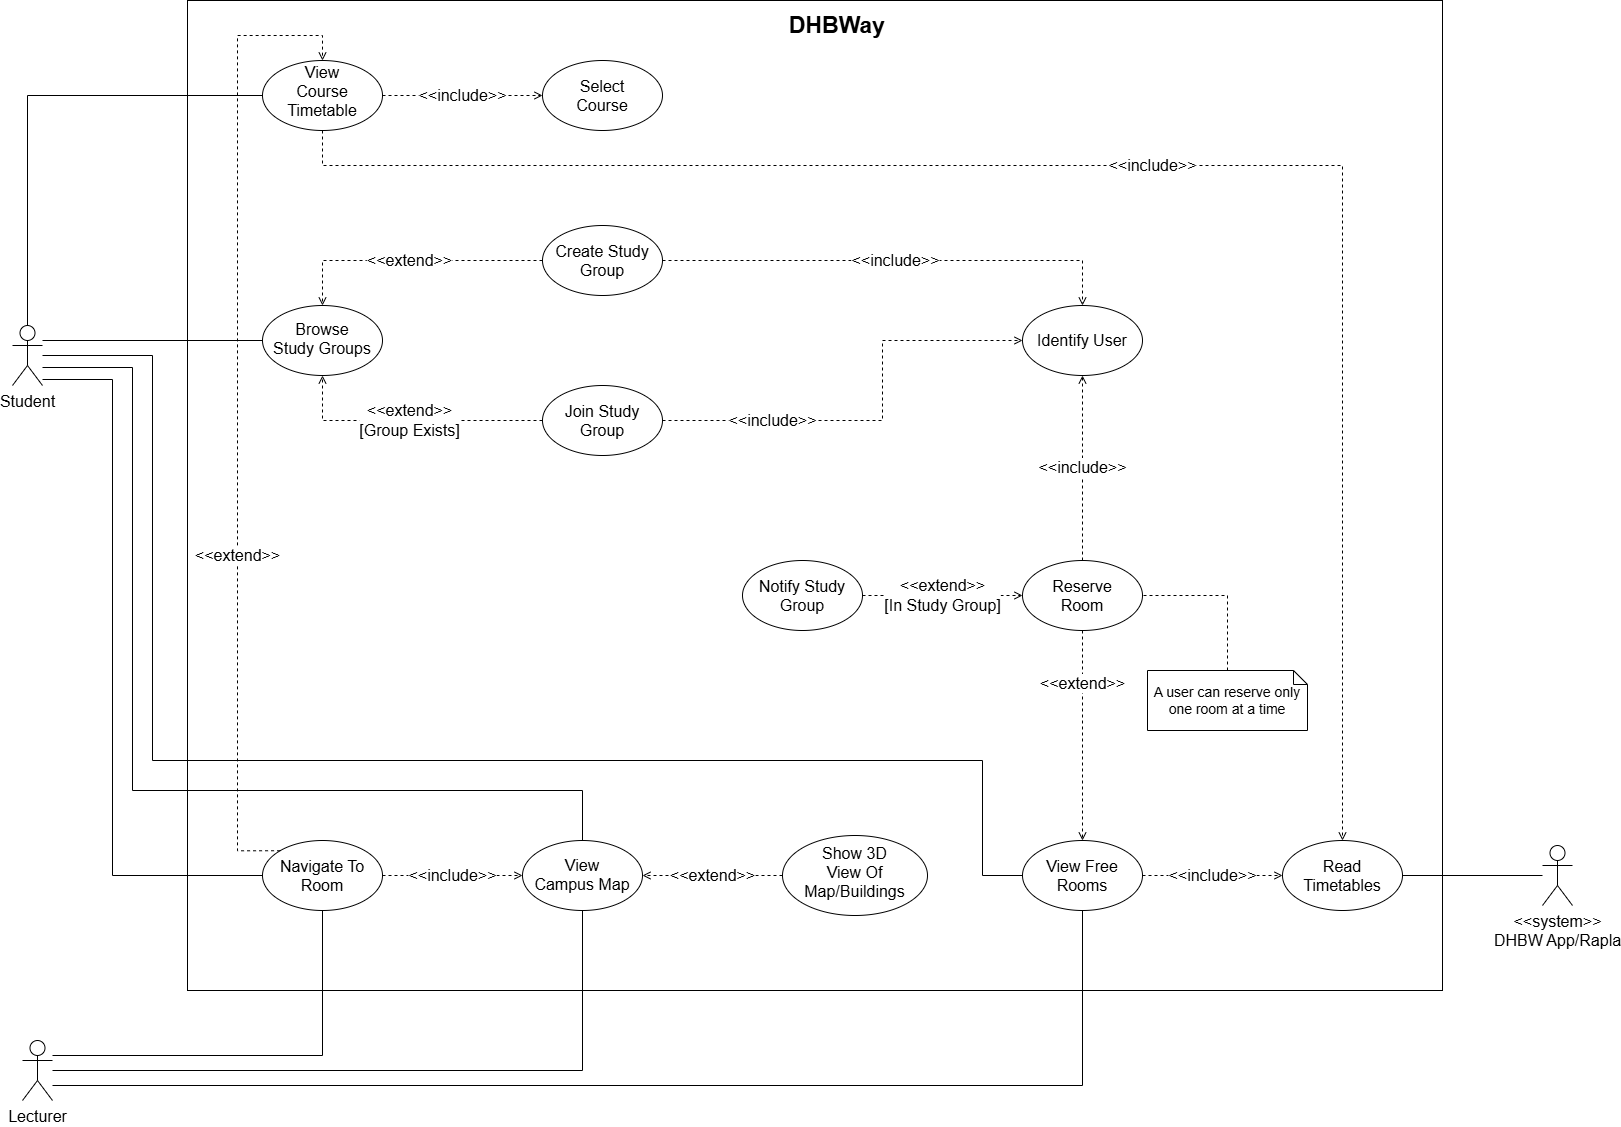
\includegraphics[width=0.98\linewidth]{Use-Case-Diagram.png}
\end{center}

\subsection*{Summary of Core Use Cases}
\begin{tabularx}{\textwidth}{l l X}
    \toprule
    \textbf{Use Case} & \textbf{Primary Actor(s)} & \textbf{High-Level Goal} \\
    \midrule
    UC-1: Timetable & Students & Organized view of their timetable \\
    UC-2: Study Groups & Students & Create and join Study groups \\
    UC-3: Free Rooms & Students \& Lecturers & Find rooms that are unused \& reserve them for self-study or the study group \\
    UC-4: Campus Map & Students \& Lecturers & View a map of the campus (2D \& 3D) \\
    UC-5: Campus Navigation & Students \& Lecturers & Navigation to a selected room on the map \\

    \bottomrule
\end{tabularx}

\end{document}